\documentclass[dvipdfmx]{article}
\usepackage[dvipdfmx]{graphicx}
\usepackage{amsmath, amssymb}
\usepackage{mathtools}
\usepackage{here}
\usepackage{color}

\begin{document}
\title{Weekly Report}
\author{Riku Gondow}
\maketitle
\section{Progress}
\begin{itemize}
    \item Reimplement Inception Time\cite{Inception}, Xing-San used as a baseline method. (almost finished)

    I am currently asking Xing-San questions about what is not working.

    \item \textcolor{red}{Finished reimplementing InceptionTime for close-set identification}
\end{itemize}

\section{\textcolor{red}{Human identification based on 1D-CNN (InceptionTime)}}

\begin{figure}[H]
\begin{center}
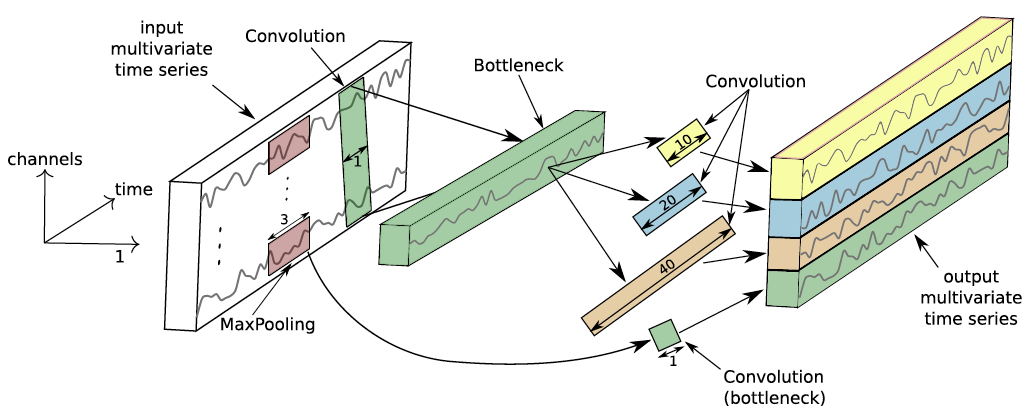
\includegraphics[width=0.8\linewidth]{./img/Incep.png}
\end{center}
\caption{The architecture of InceptionTime}
\end{figure}

Using a model called Inception Time, we tried identifying 30 subjects using heartbeat signals generated from radar.
We split the data 8:2, and used 4330 instances for training, 1083 instances for test.
Table 1 shows the hyper parameters and Figure 2 shows the confusion matrix.
We achieved 99.08\% accuracy on close-set.

\begin{table}[H]
\caption{Hyper parameter}
\centering
\begin{tabular}{cc}
\hline
batch size & 64 \\
learning rate & 0.001 \\
epochs & 10 \\
Sampling rate & 250 Hz \\
window size & 5s \\
overlap & 1.5s \\
\hline
\end{tabular}
\end{table}


\begin{figure}[H]
\begin{center}
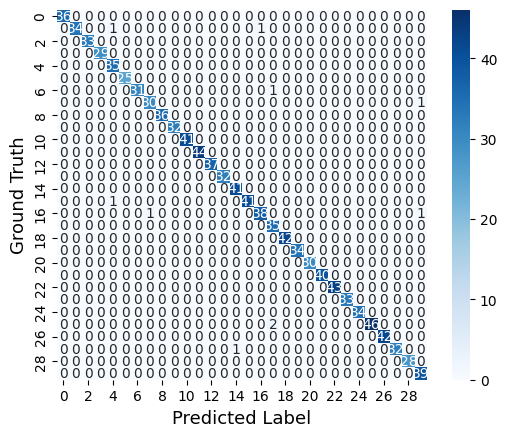
\includegraphics[width=0.8\linewidth]{./img/confu_matrix.png}
\end{center}
\caption{Confusion Matrix}
\end{figure}

\section{Next Plan}
\begin{itemize}
    \item Finish reimplementation \textcolor{red}{for Open-set}
    \item Evaluate the performance of Inception Time on the 30-subjects dataset 
\end{itemize}

\begin{thebibliography}{99}
\bibitem{Inception} Ismail Fawaz, H., Lucas, B., Forestier, G. et al. InceptionTime: Finding AlexNet for time series classification. Data Min Knowl Disc 34, 1936–1962 (2020). https://doi.org/10.1007/s10618-020-00710-y
\end{thebibliography}
\end{document}